%% ------------------------------------------------------------------------- %%
\chapter{Gradient Boosting Machines}
\label{cap:boosting-intro}

\textit{Gradient Boosting Machines}(GBM) is a machine learning algorithm, based on the idea of additive models from statistics and gradient descent. GBM works by building a forward stagewise additive model by performing gradient descent in function space, as proposed by \cite{gbmdef}. The \textit{Additive Modelling} technique and the \textit{Gradient Descent} algorithm are key ideas to GBMs, and will be briefly introduced below.

\section{Additive Model}\index{additive!model}\index{regression}
An additive model is a  regression technique suggested by \sloppy{\cite{doi:10.1080/01621459.1981.10477729}}, where the basic idea is to approximate a dataset using a sum of \textbf{smooth functions} of the individual features of the observed data, instead of a complex general regression surface.

Consider a supervised dataset is a set of pairs $\supervised$, where $\xisup$ denotes the $p$-dimensional vector of the $i$-th observation ($p$ is the number of features), and $\yisup$ is the true outcome of the $i$-th observation. An additive model is then described as:

\begin{equation}\label{eq:additive}
\mathbb{E}[\yisup\mid \xisup] = \beta_0 + \sum_{j=1}^pf_j(\xmat_{:, j})
\end{equation}

The $\beta_0$ is the intercept term, and each function $f_j$ is learned from the respective $j$-th feature over all the observations in the dataset. Each of those functions can be estimated using any nonparametric regression technique, such as Gaussian Process Regression, smoothing splines, kernel regression, k-nearest-neighbors, etc.

\section{Gradient Descent}\index{gradient!descent}\index{descent}
\label{Gradient Descent}

Gradient Descent is an iterative optimization algorithm. As explained by \cite{Ruder2016AnOO}, the basic version of the algorithm is used to \textbf{minimize} an objective function $J(\xmat;\theta)$, parameterized by a model's parameters $\theta \in \mathbb{R}^p$, by using the information gradient vector w.r.t the parameters $\theta$ of the function at a specific point to update the parameters in the opposite direction of this vector. Usually the parameters $\theta$ are updated until a fixed number of iterations is reached, or a convergence is reached. This algorithm uses the learning rate $\eta$ to control how much the coefficients of $\theta$ can change on each iteration.

The basic update rule of the original gradient descent algorithm is defined as

$$\theta_t = \theta_{t-1} - \eta \cdot \nabla_{\theta_{t-1}} J(\xmat;\theta_{t-1})$$

A gradient descent execution will run the above update $M$ times, and it can be interpreted as generating $M$ vectors $p_m$ of the form $p_m = -\eta\cdot\nabla_{\theta_{m-1}}J(\xmat;\theta_{m-1})$, and  This is a key idea which is important in the mathematical formulation of Gradient Boosting Machines. 
Denoting $p_0 = \theta_0$ (the initial parameters values before optimization), the final optimal parameters $\theta^\star$ can be written as

\begin{equation}
    \theta^\star = \sum_{m=0}^{M}p_m
\end{equation}

\section{Boosting and \textit{AdaBoost}}\index{boosting}\index{AdaBoost}\index{boost}

The boosting method is a general technique which attempts to "boost" the accuracy of a given machine learning algorithm, answering the following question: "Can a set of weak learners create a single strong learner?". A \textit{weak learner} is a model that performs just slightly better than random guessing. The purpose of boosting is to sequentially apply the \textit{weak learning algorithm} (i.e. an algorithm that produces \textit{weak learners}) to modified versions of the data, producing a sequence of weak classifiers $f_m(x), m = 1, 2, ..., M$, as described by \cite{hastie2009elements}. 

In a superficial level, boosting is similar to another technique called \textit{bagging}, used in the famous \textit{Random Forest} learning algorithm, as both are trying to create a strong learner from an ensemble of weak learners. However, they are fundamentally different: In both bagging and boosting, the variance of the estimates are reduced when the ensemble of learners is created, however the boosting method reduces both the bias and the variance, which makes this technique prone to \textit{overfitting}.

\cite{Schapire:1999:BIB:1624312.1624417} gives a brief overview of the boosting method and its applications, especially the famous \textbf{AdaBoost} algorithm, which was a major breakthrough in Machine Learning research. The original AdaBoost algorithm is designed for classification problems, where the output is either $-1$ or $1$, and the final prediction for a given instance is a weighted sum of each generated weak classifier:

\begin{equation}\label{eq:boosting}
    F_m(x) = sign(\sum_{m=1}^{M}\rho_m\cdot f_m(x))
\end{equation}

The weights $\rho_m$ in equation \ref{eq:boosting} are computed by the boosting algorithm, and the idea is increase the influence of weak learners that are more accurate, while at the same time penalizing the ones that do not predict very well. 

The data modifications done in each step of the boosting procedure is to assign weights $w_i$ for each $\xisup$ in the dataset, based if the instance $\xisup$ was correctly classified or not. The initial weight for all data points is $1/n$, and in the boosting process these weights are adjusted following an exponential function using $\rho_m$ and if the point being updated was correctly classified or not in the last update. One can refer to \cite{hastie2009elements} for a detailed explanation of the AdaBoost algorithm and its formal mathematical description. 

\begin{figure}[!h]
  \centering
  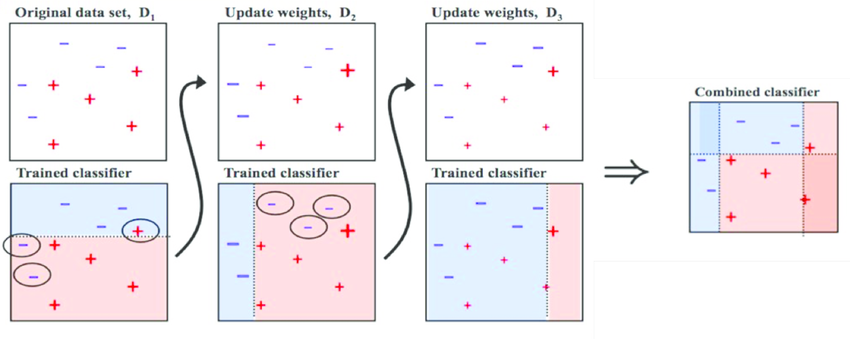
\includegraphics[width=.80\textwidth]{adaboost_classifier.png} 
  \caption{Training of an AdaBoost classifier, image from \cite{adaboost:brendan}}
  \label{fig:humanbeta} 
\end{figure}

\section{GBMs}\index{boosting}\index{gradient!boosting!machines}\index{boost}

Gradient Boosting Machines were originally introduced by \cite{gbmdef}, in the paper titled "Greedy Function Approximation: A Gradient Boosting Machine". In this work, Friedman makes a connection between stagewise additive expansions (concept of an additive model) and gradient descent. The GBM algorithm works by optimizing any given differentiable loss function, using gradient descent. However, the optimization is not done in terms of a numeric optimization (i.e. of updating a vector of parameters $\theta$), as described in the \ref{Gradient Descent} section, but by "boosting" functions in the direction of the gradient of the loss function.

Since GBMs deal with finite data, they optimize the functions in terms of the supervised dataset $\supervised$ inputs, not w.r.t all values of $x$, as they're (usually) infinite. The final model of the GBM will be similar to equations \ref{eq:additive} and \ref{eq:boosting}:

\begin{equation}\label{eq:gbm-1}
    F_M(x) = F_0(x) + \sum_{m=1}^M F_m(x)
\end{equation}

The $F_m(x)$ functions are boosted functions built in a stagewise fashion, just like the $\theta_t$ in gradient descent. The base functions are learners, and they can be paremeterized as $\beta_mh(x;a_m)$, where $\beta_m$ is a weight, and $a_m$ the learner parameters. Also, given a loss function $L(y_i, F_m(x_i))$, we would like to find all the optimal values of $a_m$ and $\beta_m$ that would minimize the loss function, ie., if we have $M$ functions:

\begin{equation*}
\{\beta_m, a_m\}_1^M = \argmin_{\{\beta_m^\apsimple, a_m^\apsimple\}_1^M} \sum_{i=1}^n L\bigg(\yisup, \sum_{m=1}^M \beta_m^\apsimple h(\xisup;a_m^\apsimple)\bigg)
\end{equation*}

However in most situations the optimization above is infeasible, so the \say{greedy-stagewise} approach is to optimize each pair $(\beta_m, a_m)$ in a stagewise model, that is, for each $m = 1, 2, ..., M$

\begin{equation*}
    (\beta_m, a_m) = \argmin_{\beta, a} \sum_{i=1}^n L(\yisup, F_{m-1}(\xisup) + \beta h(\xisup; a))
\end{equation*}

and the update rule of the $F_m$ functions described in \ref{eq:gbm-1} is

\begin{equation}
    F_m(x) = F_{m-1}(x) + \beta_m h(x; a_m)
\end{equation}

Para a escrita de textos em Ciência da Computação, o livro de Justin Zobel, 
\emph{Writing for Computer Science} \cite{zobel:04} é uma leitura obrigatória. 
O livro \emph{Metodologia de Pesquisa para Ciência da Computação} de 
Raul Sidnei Wazlawick \cite{waz:09} também merece uma boa lida.
Já para a área de Matemática, dois livros recomendados são o de Nicholas Higham,
\emph{Handbook of Writing for Mathematical Sciences} \cite{Higham:98} e o do criador
do \TeX, Donald Knuth, juntamente com Tracy Larrabee e Paul Roberts, 
\emph{Mathematical Writing} \cite{Knuth:96}.

O uso desnecessário de termos em lingua estrangeira deve ser evitado. No entanto,
quando isso for necessário, os termos devem aparecer \emph{em itálico}.

\begin{small}
\begin{verbatim}
Modos de citação:
indesejável: [AF83] introduziu o algoritmo ótimo.
indesejável: (Andrew e Foster, 1983) introduziram o algoritmo ótimo.
certo : Andrew e Foster introduziram o algoritmo ótimo [AF83].
certo : Andrew e Foster introduziram o algoritmo ótimo (Andrew e Foster, 1983).
certo : Andrew e Foster (1983) introduziram o algoritmo ótimo.
\end{verbatim}
\end{small}

Uma prática recomendável na escrita de textos é descrever as legendas das
figuras e tabelas em forma auto-contida: as legendas devem ser razoavelmente
completas, de modo que o leitor possa entender a figura sem ler o texto onde a
figura ou tabela é citada.  

Apresentar os resultados de forma simples, clara e completa é uma tarefa que
requer inspiração. Nesse sentido, o livro de Edward Tufte \cite{tufte01:visualDisplay},
\emph{The Visual Display of Quantitative Information}, serve de ajuda na 
criação de figuras que permitam entender e interpretar dados/resultados de forma
eficiente.

% \emph{Thesis are random access. Do NOT feel obliged to read a thesis from beginning to end.}



%% ------------------------------------------------------------------------- %%
\section{Considerações Preliminares}
\label{sec:consideracoes_preliminares}

Considerações preliminares\footnote{Nota de rodapé (não abuse).}\index{genoma!projetos}.
% index permite acrescentar um item no indice remissivo
Texto texto texto texto texto texto texto texto texto texto texto texto texto
texto texto texto texto texto texto texto texto texto texto texto texto texto
texto texto texto texto texto texto texto.
 

%% ------------------------------------------------------------------------- %%
\section{Objetivos}
\label{sec:objetivo}

Texto texto texto texto texto texto texto texto texto texto texto texto texto
texto texto texto texto texto texto texto texto texto texto texto texto texto
texto texto texto texto texto texto.

%% ------------------------------------------------------------------------- %%
\section{Contribuições}
\label{sec:contribucoes}

As principais contribuições deste trabalho são as seguintes:

\begin{itemize}
  \item Item 1. Texto texto texto texto texto texto texto texto texto texto
  texto texto texto texto texto texto texto texto texto texto.

  \item Item 2. Texto texto texto texto texto texto texto texto texto texto
  texto texto texto texto texto texto texto texto texto texto.

\end{itemize}

%% ------------------------------------------------------------------------- %%
\section{Organização do Trabalho}
\label{sec:organizacao_trabalho}

No Capítulo~\ref{cap:boosting-intro}, apresentamos os conceitos ... Finalmente, no
Capítulo~\ref{cap:boosting-intro} discutimos algumas conclusões obtidas neste
trabalho. Analisamos as vantagens e desvantagens do método proposto ... 

As sequências testadas no trabalho estão disponíveis no Apêndice \ref{ape:sequencias}.
